\documentclass[11pt,a4paper]{article}
\usepackage[utf8]{inputenc}
\usepackage[T1]{fontenc}
\usepackage{amsthm} %numéroter les questions
\usepackage[english]{babel}
\usepackage{datetime}
\usepackage{xspace} % typographie IN
\usepackage{hyperref}% hyperliens
\usepackage[all]{hypcap} %lien pointe en haut des figures

\usepackage{fancyhdr}% en têtes
\usepackage{graphicx} %include pictures
\usepackage{pgfplots}

% \usepackage{minted}
\usepackage{colortbl}
\usepackage{tikz}
\usetikzlibrary{calc}
\usetikzlibrary{babel}
\usetikzlibrary{tikzmark}

\usepackage{circuitikz}
% \usepackage{gnuplottex}
\usepackage{float}
\usepackage{ifthen}

\usepackage[top=1.3 in, bottom=1.3 in, left=1.3 in, right=1.3 in]{geometry}
\usepackage[]{pdfpages}
\usepackage[]{attachfile}

\usepackage{amsmath}
\usepackage{enumitem}
\setlist[enumerate]{label=\alph*)}% If you want only the x-th level to use this format, use '[enumerate,x]'
\usepackage{multirow}

\usepackage{aeguill} %guillemets


%%%%%%%%%%%%%%%%%%%%%%%%%%%%%%%%%%%%%%%%%%%%%%%%%%%%%%%%%%%%%%%%%%%%%%%%%%%%%%%%%%%%%%%%%%%
% READ THIS BEFORE CHANGING ANYTHING
%
%
% - TP number: can be changed using the command
%		\def \tpnumber {TP 1 }
%
% - Version: controlled by a new command:
%		\newcommand{\version}{v1.0.0}
%
% - Booleans: there are three booleans used in this document:
%	- 'corrige', controlled by defining the variable 'corrige'
% You can define those variables in a makefile using such a command:
% pdflatex -shell-escape -jobname="infoh410_tp1" "\def\corrige{} \documentclass[11pt,a4paper]{article}
\usepackage[utf8]{inputenc}
\usepackage[T1]{fontenc}
\usepackage{amsthm} %numéroter les questions
\usepackage[english]{babel}
\usepackage{datetime}
\usepackage{xspace} % typographie IN
\usepackage{hyperref}% hyperliens
\usepackage[all]{hypcap} %lien pointe en haut des figures
%\usepackage[french]{varioref} %voir x p y

\usepackage{fancyhdr}% en têtes
\usepackage{graphicx} %include pictures
\usepackage{pgfplots}

\usepackage{minted}
\usepackage{tikz}
\usetikzlibrary{calc}
\usetikzlibrary{babel}
\usepackage{circuitikz}
% \usepackage{gnuplottex}
\usepackage{float}
\usepackage{ifthen}

\usepackage[top=1.3 in, bottom=1.3 in, left=1.3 in, right=1.3 in]{geometry}
\usepackage[]{pdfpages}
\usepackage[]{attachfile}

\usepackage{amsmath}
\usepackage{enumitem}
\setlist[enumerate]{label=\alph*)}% If you want only the x-th level to use this format, use '[enumerate,x]'
\usepackage{multirow}

\usepackage{aeguill} %guillemets


%%%%%%%%%%%%%%%%%%%%%%%%%%%%%%%%%%%%%%%%%%%%%%%%%%%%%%%%%%%%%%%%%%%%%%%%%%%%%%%%%%%%%%%%%%%
% READ THIS BEFORE CHANGING ANYTHING
%
%
% - TP number: can be changed using the command
%		\def \tpnumber {TP 1 }
%
% - Version: controlled by a new command:
%		\newcommand{\version}{v1.0.0}
%
% - Booleans: there are three booleans used in this document:
%	- 'corrige', controlled by defining the variable 'corrige'
% You can define those variables in a makefile using such a command:
% pdflatex -shell-escape -jobname="infoh410_tp1" "\def\corrige{} \documentclass[11pt,a4paper]{article}
\usepackage[utf8]{inputenc}
\usepackage[T1]{fontenc}
\usepackage{amsthm} %numéroter les questions
\usepackage[english]{babel}
\usepackage{datetime}
\usepackage{xspace} % typographie IN
\usepackage{hyperref}% hyperliens
\usepackage[all]{hypcap} %lien pointe en haut des figures
%\usepackage[french]{varioref} %voir x p y

\usepackage{fancyhdr}% en têtes
\usepackage{graphicx} %include pictures
\usepackage{pgfplots}

\usepackage{minted}
\usepackage{tikz}
\usetikzlibrary{calc}
\usetikzlibrary{babel}
\usepackage{circuitikz}
% \usepackage{gnuplottex}
\usepackage{float}
\usepackage{ifthen}

\usepackage[top=1.3 in, bottom=1.3 in, left=1.3 in, right=1.3 in]{geometry}
\usepackage[]{pdfpages}
\usepackage[]{attachfile}

\usepackage{amsmath}
\usepackage{enumitem}
\setlist[enumerate]{label=\alph*)}% If you want only the x-th level to use this format, use '[enumerate,x]'
\usepackage{multirow}

\usepackage{aeguill} %guillemets


%%%%%%%%%%%%%%%%%%%%%%%%%%%%%%%%%%%%%%%%%%%%%%%%%%%%%%%%%%%%%%%%%%%%%%%%%%%%%%%%%%%%%%%%%%%
% READ THIS BEFORE CHANGING ANYTHING
%
%
% - TP number: can be changed using the command
%		\def \tpnumber {TP 1 }
%
% - Version: controlled by a new command:
%		\newcommand{\version}{v1.0.0}
%
% - Booleans: there are three booleans used in this document:
%	- 'corrige', controlled by defining the variable 'corrige'
% You can define those variables in a makefile using such a command:
% pdflatex -shell-escape -jobname="infoh410_tp1" "\def\corrige{} \documentclass[11pt,a4paper]{article}
\usepackage[utf8]{inputenc}
\usepackage[T1]{fontenc}
\usepackage{amsthm} %numéroter les questions
\usepackage[english]{babel}
\usepackage{datetime}
\usepackage{xspace} % typographie IN
\usepackage{hyperref}% hyperliens
\usepackage[all]{hypcap} %lien pointe en haut des figures
%\usepackage[french]{varioref} %voir x p y

\usepackage{fancyhdr}% en têtes
\usepackage{graphicx} %include pictures
\usepackage{pgfplots}

\usepackage{minted}
\usepackage{tikz}
\usetikzlibrary{calc}
\usetikzlibrary{babel}
\usepackage{circuitikz}
% \usepackage{gnuplottex}
\usepackage{float}
\usepackage{ifthen}

\usepackage[top=1.3 in, bottom=1.3 in, left=1.3 in, right=1.3 in]{geometry}
\usepackage[]{pdfpages}
\usepackage[]{attachfile}

\usepackage{amsmath}
\usepackage{enumitem}
\setlist[enumerate]{label=\alph*)}% If you want only the x-th level to use this format, use '[enumerate,x]'
\usepackage{multirow}

\usepackage{aeguill} %guillemets


%%%%%%%%%%%%%%%%%%%%%%%%%%%%%%%%%%%%%%%%%%%%%%%%%%%%%%%%%%%%%%%%%%%%%%%%%%%%%%%%%%%%%%%%%%%
% READ THIS BEFORE CHANGING ANYTHING
%
%
% - TP number: can be changed using the command
%		\def \tpnumber {TP 1 }
%
% - Version: controlled by a new command:
%		\newcommand{\version}{v1.0.0}
%
% - Booleans: there are three booleans used in this document:
%	- 'corrige', controlled by defining the variable 'corrige'
% You can define those variables in a makefile using such a command:
% pdflatex -shell-escape -jobname="infoh410_tp1" "\def\corrige{} \input{infoh410_tp1.tex}"
%
%%%%%%%%%%%%%%%%%%%%%%%%%%%%%%%%%%%%%%%%%%%%%%%%%%%%%%%%%%%%%%%%%%%%%%%%%%%%%%%%%%%%%%%%%%%

%Numero du TP :
\def \tpnumber {TP 1 \& 2}

\newcommand{\version}{v1.0.0}


% ########     #####      #####    ##         #########     ###     ##      ##  
% ##     ##  ##     ##  ##     ##  ##         ##           ## ##    ###     ##  
% ##     ##  ##     ##  ##     ##  ##         ##          ##   ##   ## ##   ##  
% ########   ##     ##  ##     ##  ##         ######     ##     ##  ##  ##  ##  
% ##     ##  ##     ##  ##     ##  ##         ##         #########  ##   ## ##  
% ##     ##  ##     ##  ##     ##  ##         ##         ##     ##  ##     ###  
% ########     #####      #####    #########  #########  ##     ##  ##      ##  
\newboolean{corrige}
\ifx\correction\undefined
\setboolean{corrige}{false}% pas de corrigé
\else
\setboolean{corrige}{true}%corrigé
\fi

\setboolean{corrige}{true}% pas de corrigé


\definecolor{darkblue}{rgb}{0,0,0.5}

\pdfinfo{
/Author (ULB -- CoDe/IRIDIA)
/Title (\tpnumber, INFO-H-410)
/ModDate (D:\pdfdate)
}

\hypersetup{
pdftitle={\tpnumber [INFO-H-410] Techniques of AI},
pdfauthor={ULB -- CoDe/IRIDIA},
pdfsubject={}
}

\theoremstyle{definition}% questions pas en italique
\newtheorem{Q}{Question}[] % numéroter les questions [section] ou non []


%  ######     #####    ##       ##  ##       ##     ###     ##      ##  ######      #######   
% ##     ##  ##     ##  ###     ###  ###     ###    ## ##    ###     ##  ##    ##   ##     ##  
% ##         ##     ##  ## ## ## ##  ## ## ## ##   ##   ##   ## ##   ##  ##     ##  ##         
% ##         ##     ##  ##  ###  ##  ##  ###  ##  ##     ##  ##  ##  ##  ##     ##   #######   
% ##         ##     ##  ##       ##  ##       ##  #########  ##   ## ##  ##     ##         ##  
% ##     ##  ##     ##  ##       ##  ##       ##  ##     ##  ##     ###  ##    ##   ##     ##  
%  #######     #####    ##       ##  ##       ##  ##     ##  ##      ##  ######      #######   
\newcommand{\reponse}[1]{% pour intégrer une réponse : \reponse{texte} : sera inclus si \boolean{corrige}
\ifthenelse {\boolean{corrige}} {\paragraph{Answer:} \color{darkblue}   #1\color{black}} {}
}

\newcommand{\addcontentslinenono}[4]{\addtocontents{#1}{\protect\contentsline{#2}{#3}{#4}{}}}


%  #######   ##########  ##    ##   ##         #########  
% ##     ##      ##       ##  ##    ##         ##         
% ##             ##        ####     ##         ##         
%  #######       ##         ##      ##         ######     
%        ##      ##         ##      ##         ##         
% ##     ##      ##         ##      ##         ##         
%  #######       ##         ##      #########  #########  
%% fancy header & foot
\pagestyle{fancy}
\lhead{[INFO-H-410] Techniques of AI\\ \tpnumber}
\rhead{\version\\ page \thepage}
\chead{\ifthenelse{\boolean{corrige}}{Correction}{}}
\cfoot{}
%%

\setlength{\parskip}{0.2cm plus2mm minus1mm} %espacement entre §
\setlength{\parindent}{0pt}

% ##########  ########   ##########  ##         #########  
%     ##         ##          ##      ##         ##         
%     ##         ##          ##      ##         ##         
%     ##         ##          ##      ##         ######     
%     ##         ##          ##      ##         ##         
%     ##         ##          ##      ##         ##         
%     ##      ########       ##      #########  ######### 
\date{\vspace{-1.7cm}\version}
\title{\vspace{-2cm} \tpnumber \\ Techniques of AI [INFO-H-410] \ifthenelse{\boolean{corrige}}{~\\Correction}{}}


\begin{document}
\selectlanguage{english}

\maketitle
\paragraph{Fundamentals for search}
\begin{Q}
Suppose you have a data structure D with the push and pop operation. Suppose you have
the following sequence of push operations: push(1), push(3), push(2).

\begin{enumerate}
    \item Which elements are returned by two consecutive pop operations if D is a stack, if D is a queue?
    \item Now suppose that D is a priority queue and that the priority of each element is the value 
        of the element itself. Which elements are returned by two consecutive pop operations now?
\end{enumerate}
Use python to validate your answers.

\reponse{
    (a) If D is a stack, the first pop operation returns 2, the second one returns 3. If D is a
queue, the first pop operation returns 1, the second one returns 3.

(b) If D is a priority queue, the first pop operation returns 3, the second one returns 2.
}

\end{Q}


\paragraph{General search algorithms}

\begin{Q}
The outline of a general tree search algorithm is sketched below. How can this outline be
turned into:
\begin{enumerate}
    \item depth first search
    \item breadth first search
    \item best first search
    \item A* search
\end{enumerate}

\begin{minted}[frame=lines,framesep=5pt,linenos]{python3}
q = [start]
while len(q) != 0:
    current = q.pop()
    if current == goal:
        print("Found goal")
        break
    for n in neighbors(current):
        q.append(n)
\end{minted}

For each of those search algorithms, start from the general algorithm above and add more
details to it, such that it becomes the desired search algorithm.
\reponse{
(a) for depth first search, the agenda should operate as a stack: new nodes are added to
the front of the agenda and taken from the front.

(b) for breadth first search, the agenda should operate as a queue

(c) for best first search, the agenda should be a priority queue with priorities f(n) = h(n)

(d) for A*, the agenda should be a priority queue with priorities f(n) = g(n) + h(n)
}
\end{Q}


\paragraph{Search spaces}
\begin{Q}
Consider the following state space:
\begin{center}
\begin{tikzpicture}[node distance={25mm}, main/.style = {draw, circle}] 
\node[main] (1) {$S (10)$}; 
\node[main] (2) [below left of=1] {$A (5)$}; 
\node[main] (3) [below right of=1] {$B (8)$}; 
\node[main] (4) [left of=2] {$C (3)$}; 
\node[main] (5) [below of=2]{$D (2)$}; 
\node[main] (6) [below of=3] {$E (4)$}; 
\node[main] (7) [below of=4] {$G_1 (0)$}; 
\node[main] (8) [right of=3]{$G_2 (0)$}; 
\draw[->] (1) -- node[below right]{3} (2);
\draw[->] (1) -- node[above]{7} (3);
\draw[->] (2) -- node[right]{6} (5);
\draw[->] (2) -- node[above]{1} (4);
\draw[->] (3) -- node[above]{9} (8);
\draw[->] (3) -- node[left]{1} (6);
\draw[->] (4) -- node[above]{4} (5);
\draw[->] (4) -- node[above]{2} (1);
\draw[->] (5) -- node[above]{6} (7);
\draw[->] (5) -- node[above]{3} (3);
\draw[->] (6) -- node[above]{5} (8);
\draw[->] (7) -- node[left]{2} (4);
\draw[->] (8) to[in=90] node[above]{8} (3);
\end{tikzpicture} 
\end{center}

\begin{itemize}
    \item S is the initial state 
    \item G1 and G2 are goal states
    \item Arcs show actions between states (e.g., the successor function for state S returns {A,
    B}).
    \item Arcs are labelled with actual cost of the action (e.g. the action from S to A has a cost
    of 3).
    \item The numeric value in parentheses in each state is the states h-value (e.g. $h(A) = 5$).
\end{itemize}
You should assume the following on the operational details of the algorithms:

\begin{itemize}
    \item The algorithm does not check if a state is revisited, so there may be several nodes with
    the same state in the search tree.
    \item The algorithm terminates only when it selects a goal node for expansion, not when it
    is generated by the successor function.
    \item The successor function always orders states alphabetically.
\end{itemize}

\begin{enumerate}
    \item Give the sequence of states that will be visited, together with the total cost 
        of reaching the goal state, for (1) depth first search, (2) breadth first search 
        and (3) A*.
    \item In python what data structure could be used to store this graph ? 
        Implement one of the 3 algorithms in python and verify your previous answers 
        (you can use the following template).
\end{enumerate}

\begin{minted}[frame=lines,framesep=5pt,linenos]{python3}
def q3():
    """the graph can be stored using a adjency list or an adjency matrix.
    Usually, the matrix is easier to use but uses more memory, here 
    we use an adjency list."""
    # we store states as indexes in the list, where S->0, A->1, B->2 etc.
    # each sublist represents the list all states to which state i 
    # is connected, with associated cost.
    graph = [
        [(2, 7), (1, 3)], # S (linked to 2(B) with cost 7, and 1(A) cost 3)
        [(4, 6), (3, 1)], # A
        [(7, 9), (5, 1)], # B
        [(0, 2), (4, 4)], # C
        [(6, 6), (2, 3)], # D
        [(7, 5)], # E
        [(3, 2)], # G1
        [(2, 8)], # G2
    ]
    h = [10, 5, 8, 3, 2, 4, 0, 0]

\end{minted}


\reponse{
Depth first search, path found: S – A – C – D – B – E – G2 = 17
Breadth first search, path found: S – B – G2 = 16
A*, path found: S – A – C – D – G1 = 14
}
\end{Q}

\paragraph{ The Missionaries and Cannibals Puzzle}
\begin{Q}
    There are three missionaries and three cannibals on the west bank of a river. There is a
boat on the west bank that can hold no more than two people. The missionaries wish to
cross to the east bank. But they have a problem: If on either bank the cannibals ever
outnumber the missionaries, the outnumbered missionaries will be eaten. Is there a way for
the missionaries to get to the east bank without losing anyone?

\begin{enumerate}
    \item Represent this puzzle as a search problem by defining the states and actions.
    \item Investigate your initial representation of the puzzle as you did in part (a): is there
any redundant information in your representation? Try to remove any redundant
information from it.
    \item Try to solve the puzzle by enumerating possible states.
    \item Implement and solve the puzzle using python. 
\end{enumerate}

\reponse{
    (a) A straightforward approach would be to represent the state by an array containing the
following:
•
 number of missionaries at the left
•
 number of cannibals at the left
•
 number of missionaries at the right
•
 number of cannibals at the right
•
 number of missionaries in the boat
•
 number of cannibals in the boat
•
 position of the boat
(b) This representation is overcomplete: if you know how many missionaries and cannibals
we have at the one bank and in the boat, we know how many there are at the other
bank, as we always have 3 missionaries and 3 cannibals. So, a first improvement might
be the following representation:
•
 number of missionaries at the left
•
 number of cannibals at the left
•
 number of missionaries in the boat
•
 number of cannibals in the boat
•
 position of the boat
However, as the boat can contain at most 1 missionary and 1 cannibal, the cannibals
can never outnumber the missionaries in the boat, so it is of no use to represent the
number of each in the boat. So, we could simply store:
• number of missionaries at the left
• number of cannibals at the left
• position of the boat
For instance < 3, 3, 1 > represent the initial state, with 3 missionaries and 3 cannibals
at the left bank, with the boat at the left bank. The state< 3, 1, 0 > can then be
reached from this state, by the action“transfer two cannibals to the right bank”. As a
result, we have 3 missionaries at the left bank, one cannibal at the left bank and the
boat at the right bank.
3
(c) A state is represented by < x, y, z >, with x varying between 0 and 3, y varying between
0 and 3 and z being either 0 or 1. So, we have 4 × 4 × 2 = 32 states at most.
For the boat being at left, we can for instance list all 16 possible states: 3 3 1 / 3 2 1
/311/301/231/221/211/201/131/121/111/101/031/0
2 1/ 0 1 1 / 0 0 1.
From this list, we can eliminate the states 2 3 1 / 2 1 1 / 2 0 1 / 1 3 1 / 1 2 1 / 1 0
1 because we have more cannibals than missionaries at one bank. The same holds of
course for the boat being at the other side. So we have 3266 = 20 states.
The states < 0, 0, 1 > and < 3, 3, 0 > are not valid (because it implies that you move
an empty boat), the states < 3, 0, 1 > and < 0, 3, 0 > are not reachable, because
all preceding states are invalid: < 3, 0, 1 > can only be reached from < 2, 0, 0 > or
< 1, 0, 0 >. However, in both states the cannibals do outnumber the missionaries. In
total we have hence 16 states.
(d) One solution is the following:
< 3, 3, 1 >, < 3, 1, 0 >, < 3, 2, 1 >, < 3, 0, 0 >, < 3, 1, 1 >, < 1, 1, 0 >, < 2, 2, 1 >,
< 0, 2, 0 >, < 0, 3, 1 >, < 0, 1, 0 >, < 0, 2, 1 >, < 0, 0, 0 >

}
\end{Q}

\paragraph{Path planning}
\begin{Q}
% TODO: add figure
    Imagine a maze with some obstacles, you can only move 1 cell at a time in any of 
    the four directions (no diagonals). We have to find the shortest path from A to B.
\begin{enumerate}
    \item Discuss whether depth first search and breadth first search will always find a path from
    A to B. Will they find the shortest path?
    \item Suppose that we want to use informed search in order to guide our search. 
        What heuristic could you use ? It this heuristic admissible ?
    %We will use the Manhattan distance as a search heuristic. Discuss whether best first search will
    %find the shortest path, use the left drawing to add f, g and h costs. Will A* do so?
    %Use the right drawing to add f, g and h costs.
    \item Implement the A* algorithm for this maze using python (you can use following template).
    \item Now suppose that there is a direct underground connection from C to B. Hence, the
    shortest path from A to B now is over C (it is only five steps). Is your heuristic still admissible ?
    %Argue whether A* will find this shortest path.
\end{enumerate}

\begin{minted}[frame=lines,framesep=5pt,linenos]{python3}
def q5():
    """
    We want to find the shortest path between A and B, we are using A*.
    In A*, f = g+h is the function to minimize where g is the value of
    smallest known path and h in the heuristic
    """
    grid = [
        [0, 0, 0, 0, 0, 0],
        [0, 0, 0, 1, 0, 0],
        [0, 0, 0, 1, 0, 0],
        [0, 0, 0, 1, 0, 0],
        [0, 0, 1, 1, 0, 0],
        [0, 0, 0, 0, 0, 0],
    ]
    start = (3, 1)
    goal = (3, 4)
\end{minted}

\reponse{
    (a) If it is ensured that the algorithms do not get stuck in loops, then they will find a
solution. Depth first search will return the first path to the goal state it happens to
encounter, which is not guaranteed to be the shortest one. Breadth first search, will
find the shortest path.
(b) In this particular case, we can easily see that there are actually two possible ways of
going from A to B in an efficient manner, either travel above the obstacle or travel
below the obstacle. If you calculate the f-cost of every cell in the grid, it is observed
that both paths have exactly the same f-cost when using the best first search. However,
the lower path is shorter. So, with best first search, it is not guaranteed to find the
shortest path. With A* the shortest path is found, because the heuristic is admissible.

}
\end{Q}


\begin{Q}
    The optimality condition of A* is expressed as follows: “If the heuristic h(n) is admissible,
then the solution returned by A* is optimal”. In order to prove this, we assume that the
optimal solution n* has an optimal cost f(n*) = C*.

\begin{enumerate}
    \item Suppose that there is a solution G2 which is not optimal in the agenda. What does
    this learn about f(G2)?
    \item Suppose that there is a node n in the agenda which is on the path to the optimal
    solution G. What does this learn about f(n)?
    \item Proof that if h(n) is admissible, then the solution returned by A* is optimal.
\end{enumerate}
\reponse{
    A heuristic is admissible if it never overestimates the cost to the goal.
(a) Suppose A* returns a solution which is not optimal. This means that at some point a
non optimal solution G2 must be in the agenda. If G2 is not optimal, then f (G2) >
f (n∗) = C∗
(b) If h(n) is admissible, then h does not overestimate the cost to the goal, so we can put
f (n) < C∗
(c) Combining a and b results in the inequality: f (n) < C∗ < f (G2). Hence, every node
on the path towards the optimal solution has a cost less than the cost of the non
optimal solution G2. Hence, G2 will never be expanded from the priority queue. So,
G2 cannot be the solution of the A* algorithm.
}
\end{Q}


% \begin{Q}
% % TODO : add figure
%     A new game comes with a board which contains 7 cells (as shown below). There are 6
% pivots, each containing a number. Each pivot has to be in one cell and each cell can contain
% at most one pivot. Hence, there is always one empty cell. A pivot can be moved one cell to
% the left or one cell to the right (if it does not break the rules given above) with a cost of 1.
% A pivot can also jump over another pivot, with cost 2 (if it does not break the rules given
% above). The goal of the game is to have the empty cell in the middle, such that the sum of
% the blocks at the left of the empty cell is equal to the sum of the blocks at the right of the
% empty cell.
% \begin{enumerate}
%     \item Model this as a state space search problem.
%     \item Which of the search algorithms studied in class is best suited for solving this puzzle?
%     Motivate (max 5 lines).
%     \item Give a sequence of states leading to the goal state.
% \end{enumerate}
% \end{Q}

\end{document} 
"
%
%%%%%%%%%%%%%%%%%%%%%%%%%%%%%%%%%%%%%%%%%%%%%%%%%%%%%%%%%%%%%%%%%%%%%%%%%%%%%%%%%%%%%%%%%%%

%Numero du TP :
\def \tpnumber {TP 1 \& 2}

\newcommand{\version}{v1.0.0}


% ########     #####      #####    ##         #########     ###     ##      ##  
% ##     ##  ##     ##  ##     ##  ##         ##           ## ##    ###     ##  
% ##     ##  ##     ##  ##     ##  ##         ##          ##   ##   ## ##   ##  
% ########   ##     ##  ##     ##  ##         ######     ##     ##  ##  ##  ##  
% ##     ##  ##     ##  ##     ##  ##         ##         #########  ##   ## ##  
% ##     ##  ##     ##  ##     ##  ##         ##         ##     ##  ##     ###  
% ########     #####      #####    #########  #########  ##     ##  ##      ##  
\newboolean{corrige}
\ifx\correction\undefined
\setboolean{corrige}{false}% pas de corrigé
\else
\setboolean{corrige}{true}%corrigé
\fi

\setboolean{corrige}{true}% pas de corrigé


\definecolor{darkblue}{rgb}{0,0,0.5}

\pdfinfo{
/Author (ULB -- CoDe/IRIDIA)
/Title (\tpnumber, INFO-H-410)
/ModDate (D:\pdfdate)
}

\hypersetup{
pdftitle={\tpnumber [INFO-H-410] Techniques of AI},
pdfauthor={ULB -- CoDe/IRIDIA},
pdfsubject={}
}

\theoremstyle{definition}% questions pas en italique
\newtheorem{Q}{Question}[] % numéroter les questions [section] ou non []


%  ######     #####    ##       ##  ##       ##     ###     ##      ##  ######      #######   
% ##     ##  ##     ##  ###     ###  ###     ###    ## ##    ###     ##  ##    ##   ##     ##  
% ##         ##     ##  ## ## ## ##  ## ## ## ##   ##   ##   ## ##   ##  ##     ##  ##         
% ##         ##     ##  ##  ###  ##  ##  ###  ##  ##     ##  ##  ##  ##  ##     ##   #######   
% ##         ##     ##  ##       ##  ##       ##  #########  ##   ## ##  ##     ##         ##  
% ##     ##  ##     ##  ##       ##  ##       ##  ##     ##  ##     ###  ##    ##   ##     ##  
%  #######     #####    ##       ##  ##       ##  ##     ##  ##      ##  ######      #######   
\newcommand{\reponse}[1]{% pour intégrer une réponse : \reponse{texte} : sera inclus si \boolean{corrige}
\ifthenelse {\boolean{corrige}} {\paragraph{Answer:} \color{darkblue}   #1\color{black}} {}
}

\newcommand{\addcontentslinenono}[4]{\addtocontents{#1}{\protect\contentsline{#2}{#3}{#4}{}}}


%  #######   ##########  ##    ##   ##         #########  
% ##     ##      ##       ##  ##    ##         ##         
% ##             ##        ####     ##         ##         
%  #######       ##         ##      ##         ######     
%        ##      ##         ##      ##         ##         
% ##     ##      ##         ##      ##         ##         
%  #######       ##         ##      #########  #########  
%% fancy header & foot
\pagestyle{fancy}
\lhead{[INFO-H-410] Techniques of AI\\ \tpnumber}
\rhead{\version\\ page \thepage}
\chead{\ifthenelse{\boolean{corrige}}{Correction}{}}
\cfoot{}
%%

\setlength{\parskip}{0.2cm plus2mm minus1mm} %espacement entre §
\setlength{\parindent}{0pt}

% ##########  ########   ##########  ##         #########  
%     ##         ##          ##      ##         ##         
%     ##         ##          ##      ##         ##         
%     ##         ##          ##      ##         ######     
%     ##         ##          ##      ##         ##         
%     ##         ##          ##      ##         ##         
%     ##      ########       ##      #########  ######### 
\date{\vspace{-1.7cm}\version}
\title{\vspace{-2cm} \tpnumber \\ Techniques of AI [INFO-H-410] \ifthenelse{\boolean{corrige}}{~\\Correction}{}}


\begin{document}
\selectlanguage{english}

\maketitle
\paragraph{Fundamentals for search}
\begin{Q}
Suppose you have a data structure D with the push and pop operation. Suppose you have
the following sequence of push operations: push(1), push(3), push(2).

\begin{enumerate}
    \item Which elements are returned by two consecutive pop operations if D is a stack, if D is a queue?
    \item Now suppose that D is a priority queue and that the priority of each element is the value 
        of the element itself. Which elements are returned by two consecutive pop operations now?
\end{enumerate}
Use python to validate your answers.

\reponse{
    (a) If D is a stack, the first pop operation returns 2, the second one returns 3. If D is a
queue, the first pop operation returns 1, the second one returns 3.

(b) If D is a priority queue, the first pop operation returns 3, the second one returns 2.
}

\end{Q}


\paragraph{General search algorithms}

\begin{Q}
The outline of a general tree search algorithm is sketched below. How can this outline be
turned into:
\begin{enumerate}
    \item depth first search
    \item breadth first search
    \item best first search
    \item A* search
\end{enumerate}

\begin{minted}[frame=lines,framesep=5pt,linenos]{python3}
q = [start]
while len(q) != 0:
    current = q.pop()
    if current == goal:
        print("Found goal")
        break
    for n in neighbors(current):
        q.append(n)
\end{minted}

For each of those search algorithms, start from the general algorithm above and add more
details to it, such that it becomes the desired search algorithm.
\reponse{
(a) for depth first search, the agenda should operate as a stack: new nodes are added to
the front of the agenda and taken from the front.

(b) for breadth first search, the agenda should operate as a queue

(c) for best first search, the agenda should be a priority queue with priorities f(n) = h(n)

(d) for A*, the agenda should be a priority queue with priorities f(n) = g(n) + h(n)
}
\end{Q}


\paragraph{Search spaces}
\begin{Q}
Consider the following state space:
\begin{center}
\begin{tikzpicture}[node distance={25mm}, main/.style = {draw, circle}] 
\node[main] (1) {$S (10)$}; 
\node[main] (2) [below left of=1] {$A (5)$}; 
\node[main] (3) [below right of=1] {$B (8)$}; 
\node[main] (4) [left of=2] {$C (3)$}; 
\node[main] (5) [below of=2]{$D (2)$}; 
\node[main] (6) [below of=3] {$E (4)$}; 
\node[main] (7) [below of=4] {$G_1 (0)$}; 
\node[main] (8) [right of=3]{$G_2 (0)$}; 
\draw[->] (1) -- node[below right]{3} (2);
\draw[->] (1) -- node[above]{7} (3);
\draw[->] (2) -- node[right]{6} (5);
\draw[->] (2) -- node[above]{1} (4);
\draw[->] (3) -- node[above]{9} (8);
\draw[->] (3) -- node[left]{1} (6);
\draw[->] (4) -- node[above]{4} (5);
\draw[->] (4) -- node[above]{2} (1);
\draw[->] (5) -- node[above]{6} (7);
\draw[->] (5) -- node[above]{3} (3);
\draw[->] (6) -- node[above]{5} (8);
\draw[->] (7) -- node[left]{2} (4);
\draw[->] (8) to[in=90] node[above]{8} (3);
\end{tikzpicture} 
\end{center}

\begin{itemize}
    \item S is the initial state 
    \item G1 and G2 are goal states
    \item Arcs show actions between states (e.g., the successor function for state S returns {A,
    B}).
    \item Arcs are labelled with actual cost of the action (e.g. the action from S to A has a cost
    of 3).
    \item The numeric value in parentheses in each state is the states h-value (e.g. $h(A) = 5$).
\end{itemize}
You should assume the following on the operational details of the algorithms:

\begin{itemize}
    \item The algorithm does not check if a state is revisited, so there may be several nodes with
    the same state in the search tree.
    \item The algorithm terminates only when it selects a goal node for expansion, not when it
    is generated by the successor function.
    \item The successor function always orders states alphabetically.
\end{itemize}

\begin{enumerate}
    \item Give the sequence of states that will be visited, together with the total cost 
        of reaching the goal state, for (1) depth first search, (2) breadth first search 
        and (3) A*.
    \item In python what data structure could be used to store this graph ? 
        Implement one of the 3 algorithms in python and verify your previous answers 
        (you can use the following template).
\end{enumerate}

\begin{minted}[frame=lines,framesep=5pt,linenos]{python3}
def q3():
    """the graph can be stored using a adjency list or an adjency matrix.
    Usually, the matrix is easier to use but uses more memory, here 
    we use an adjency list."""
    # we store states as indexes in the list, where S->0, A->1, B->2 etc.
    # each sublist represents the list all states to which state i 
    # is connected, with associated cost.
    graph = [
        [(2, 7), (1, 3)], # S (linked to 2(B) with cost 7, and 1(A) cost 3)
        [(4, 6), (3, 1)], # A
        [(7, 9), (5, 1)], # B
        [(0, 2), (4, 4)], # C
        [(6, 6), (2, 3)], # D
        [(7, 5)], # E
        [(3, 2)], # G1
        [(2, 8)], # G2
    ]
    h = [10, 5, 8, 3, 2, 4, 0, 0]

\end{minted}


\reponse{
Depth first search, path found: S – A – C – D – B – E – G2 = 17
Breadth first search, path found: S – B – G2 = 16
A*, path found: S – A – C – D – G1 = 14
}
\end{Q}

\paragraph{ The Missionaries and Cannibals Puzzle}
\begin{Q}
    There are three missionaries and three cannibals on the west bank of a river. There is a
boat on the west bank that can hold no more than two people. The missionaries wish to
cross to the east bank. But they have a problem: If on either bank the cannibals ever
outnumber the missionaries, the outnumbered missionaries will be eaten. Is there a way for
the missionaries to get to the east bank without losing anyone?

\begin{enumerate}
    \item Represent this puzzle as a search problem by defining the states and actions.
    \item Investigate your initial representation of the puzzle as you did in part (a): is there
any redundant information in your representation? Try to remove any redundant
information from it.
    \item Try to solve the puzzle by enumerating possible states.
    \item Implement and solve the puzzle using python. 
\end{enumerate}

\reponse{
    (a) A straightforward approach would be to represent the state by an array containing the
following:
•
 number of missionaries at the left
•
 number of cannibals at the left
•
 number of missionaries at the right
•
 number of cannibals at the right
•
 number of missionaries in the boat
•
 number of cannibals in the boat
•
 position of the boat
(b) This representation is overcomplete: if you know how many missionaries and cannibals
we have at the one bank and in the boat, we know how many there are at the other
bank, as we always have 3 missionaries and 3 cannibals. So, a first improvement might
be the following representation:
•
 number of missionaries at the left
•
 number of cannibals at the left
•
 number of missionaries in the boat
•
 number of cannibals in the boat
•
 position of the boat
However, as the boat can contain at most 1 missionary and 1 cannibal, the cannibals
can never outnumber the missionaries in the boat, so it is of no use to represent the
number of each in the boat. So, we could simply store:
• number of missionaries at the left
• number of cannibals at the left
• position of the boat
For instance < 3, 3, 1 > represent the initial state, with 3 missionaries and 3 cannibals
at the left bank, with the boat at the left bank. The state< 3, 1, 0 > can then be
reached from this state, by the action“transfer two cannibals to the right bank”. As a
result, we have 3 missionaries at the left bank, one cannibal at the left bank and the
boat at the right bank.
3
(c) A state is represented by < x, y, z >, with x varying between 0 and 3, y varying between
0 and 3 and z being either 0 or 1. So, we have 4 × 4 × 2 = 32 states at most.
For the boat being at left, we can for instance list all 16 possible states: 3 3 1 / 3 2 1
/311/301/231/221/211/201/131/121/111/101/031/0
2 1/ 0 1 1 / 0 0 1.
From this list, we can eliminate the states 2 3 1 / 2 1 1 / 2 0 1 / 1 3 1 / 1 2 1 / 1 0
1 because we have more cannibals than missionaries at one bank. The same holds of
course for the boat being at the other side. So we have 3266 = 20 states.
The states < 0, 0, 1 > and < 3, 3, 0 > are not valid (because it implies that you move
an empty boat), the states < 3, 0, 1 > and < 0, 3, 0 > are not reachable, because
all preceding states are invalid: < 3, 0, 1 > can only be reached from < 2, 0, 0 > or
< 1, 0, 0 >. However, in both states the cannibals do outnumber the missionaries. In
total we have hence 16 states.
(d) One solution is the following:
< 3, 3, 1 >, < 3, 1, 0 >, < 3, 2, 1 >, < 3, 0, 0 >, < 3, 1, 1 >, < 1, 1, 0 >, < 2, 2, 1 >,
< 0, 2, 0 >, < 0, 3, 1 >, < 0, 1, 0 >, < 0, 2, 1 >, < 0, 0, 0 >

}
\end{Q}

\paragraph{Path planning}
\begin{Q}
% TODO: add figure
    Imagine a maze with some obstacles, you can only move 1 cell at a time in any of 
    the four directions (no diagonals). We have to find the shortest path from A to B.
\begin{enumerate}
    \item Discuss whether depth first search and breadth first search will always find a path from
    A to B. Will they find the shortest path?
    \item Suppose that we want to use informed search in order to guide our search. 
        What heuristic could you use ? It this heuristic admissible ?
    %We will use the Manhattan distance as a search heuristic. Discuss whether best first search will
    %find the shortest path, use the left drawing to add f, g and h costs. Will A* do so?
    %Use the right drawing to add f, g and h costs.
    \item Implement the A* algorithm for this maze using python (you can use following template).
    \item Now suppose that there is a direct underground connection from C to B. Hence, the
    shortest path from A to B now is over C (it is only five steps). Is your heuristic still admissible ?
    %Argue whether A* will find this shortest path.
\end{enumerate}

\begin{minted}[frame=lines,framesep=5pt,linenos]{python3}
def q5():
    """
    We want to find the shortest path between A and B, we are using A*.
    In A*, f = g+h is the function to minimize where g is the value of
    smallest known path and h in the heuristic
    """
    grid = [
        [0, 0, 0, 0, 0, 0],
        [0, 0, 0, 1, 0, 0],
        [0, 0, 0, 1, 0, 0],
        [0, 0, 0, 1, 0, 0],
        [0, 0, 1, 1, 0, 0],
        [0, 0, 0, 0, 0, 0],
    ]
    start = (3, 1)
    goal = (3, 4)
\end{minted}

\reponse{
    (a) If it is ensured that the algorithms do not get stuck in loops, then they will find a
solution. Depth first search will return the first path to the goal state it happens to
encounter, which is not guaranteed to be the shortest one. Breadth first search, will
find the shortest path.
(b) In this particular case, we can easily see that there are actually two possible ways of
going from A to B in an efficient manner, either travel above the obstacle or travel
below the obstacle. If you calculate the f-cost of every cell in the grid, it is observed
that both paths have exactly the same f-cost when using the best first search. However,
the lower path is shorter. So, with best first search, it is not guaranteed to find the
shortest path. With A* the shortest path is found, because the heuristic is admissible.

}
\end{Q}


\begin{Q}
    The optimality condition of A* is expressed as follows: “If the heuristic h(n) is admissible,
then the solution returned by A* is optimal”. In order to prove this, we assume that the
optimal solution n* has an optimal cost f(n*) = C*.

\begin{enumerate}
    \item Suppose that there is a solution G2 which is not optimal in the agenda. What does
    this learn about f(G2)?
    \item Suppose that there is a node n in the agenda which is on the path to the optimal
    solution G. What does this learn about f(n)?
    \item Proof that if h(n) is admissible, then the solution returned by A* is optimal.
\end{enumerate}
\reponse{
    A heuristic is admissible if it never overestimates the cost to the goal.
(a) Suppose A* returns a solution which is not optimal. This means that at some point a
non optimal solution G2 must be in the agenda. If G2 is not optimal, then f (G2) >
f (n∗) = C∗
(b) If h(n) is admissible, then h does not overestimate the cost to the goal, so we can put
f (n) < C∗
(c) Combining a and b results in the inequality: f (n) < C∗ < f (G2). Hence, every node
on the path towards the optimal solution has a cost less than the cost of the non
optimal solution G2. Hence, G2 will never be expanded from the priority queue. So,
G2 cannot be the solution of the A* algorithm.
}
\end{Q}


% \begin{Q}
% % TODO : add figure
%     A new game comes with a board which contains 7 cells (as shown below). There are 6
% pivots, each containing a number. Each pivot has to be in one cell and each cell can contain
% at most one pivot. Hence, there is always one empty cell. A pivot can be moved one cell to
% the left or one cell to the right (if it does not break the rules given above) with a cost of 1.
% A pivot can also jump over another pivot, with cost 2 (if it does not break the rules given
% above). The goal of the game is to have the empty cell in the middle, such that the sum of
% the blocks at the left of the empty cell is equal to the sum of the blocks at the right of the
% empty cell.
% \begin{enumerate}
%     \item Model this as a state space search problem.
%     \item Which of the search algorithms studied in class is best suited for solving this puzzle?
%     Motivate (max 5 lines).
%     \item Give a sequence of states leading to the goal state.
% \end{enumerate}
% \end{Q}

\end{document} 
"
%
%%%%%%%%%%%%%%%%%%%%%%%%%%%%%%%%%%%%%%%%%%%%%%%%%%%%%%%%%%%%%%%%%%%%%%%%%%%%%%%%%%%%%%%%%%%

%Numero du TP :
\def \tpnumber {TP 1 \& 2}

\newcommand{\version}{v1.0.0}


% ########     #####      #####    ##         #########     ###     ##      ##  
% ##     ##  ##     ##  ##     ##  ##         ##           ## ##    ###     ##  
% ##     ##  ##     ##  ##     ##  ##         ##          ##   ##   ## ##   ##  
% ########   ##     ##  ##     ##  ##         ######     ##     ##  ##  ##  ##  
% ##     ##  ##     ##  ##     ##  ##         ##         #########  ##   ## ##  
% ##     ##  ##     ##  ##     ##  ##         ##         ##     ##  ##     ###  
% ########     #####      #####    #########  #########  ##     ##  ##      ##  
\newboolean{corrige}
\ifx\correction\undefined
\setboolean{corrige}{false}% pas de corrigé
\else
\setboolean{corrige}{true}%corrigé
\fi

\setboolean{corrige}{true}% pas de corrigé


\definecolor{darkblue}{rgb}{0,0,0.5}

\pdfinfo{
/Author (ULB -- CoDe/IRIDIA)
/Title (\tpnumber, INFO-H-410)
/ModDate (D:\pdfdate)
}

\hypersetup{
pdftitle={\tpnumber [INFO-H-410] Techniques of AI},
pdfauthor={ULB -- CoDe/IRIDIA},
pdfsubject={}
}

\theoremstyle{definition}% questions pas en italique
\newtheorem{Q}{Question}[] % numéroter les questions [section] ou non []


%  ######     #####    ##       ##  ##       ##     ###     ##      ##  ######      #######   
% ##     ##  ##     ##  ###     ###  ###     ###    ## ##    ###     ##  ##    ##   ##     ##  
% ##         ##     ##  ## ## ## ##  ## ## ## ##   ##   ##   ## ##   ##  ##     ##  ##         
% ##         ##     ##  ##  ###  ##  ##  ###  ##  ##     ##  ##  ##  ##  ##     ##   #######   
% ##         ##     ##  ##       ##  ##       ##  #########  ##   ## ##  ##     ##         ##  
% ##     ##  ##     ##  ##       ##  ##       ##  ##     ##  ##     ###  ##    ##   ##     ##  
%  #######     #####    ##       ##  ##       ##  ##     ##  ##      ##  ######      #######   
\newcommand{\reponse}[1]{% pour intégrer une réponse : \reponse{texte} : sera inclus si \boolean{corrige}
\ifthenelse {\boolean{corrige}} {\paragraph{Answer:} \color{darkblue}   #1\color{black}} {}
}

\newcommand{\addcontentslinenono}[4]{\addtocontents{#1}{\protect\contentsline{#2}{#3}{#4}{}}}


%  #######   ##########  ##    ##   ##         #########  
% ##     ##      ##       ##  ##    ##         ##         
% ##             ##        ####     ##         ##         
%  #######       ##         ##      ##         ######     
%        ##      ##         ##      ##         ##         
% ##     ##      ##         ##      ##         ##         
%  #######       ##         ##      #########  #########  
%% fancy header & foot
\pagestyle{fancy}
\lhead{[INFO-H-410] Techniques of AI\\ \tpnumber}
\rhead{\version\\ page \thepage}
\chead{\ifthenelse{\boolean{corrige}}{Correction}{}}
\cfoot{}
%%

\setlength{\parskip}{0.2cm plus2mm minus1mm} %espacement entre §
\setlength{\parindent}{0pt}

% ##########  ########   ##########  ##         #########  
%     ##         ##          ##      ##         ##         
%     ##         ##          ##      ##         ##         
%     ##         ##          ##      ##         ######     
%     ##         ##          ##      ##         ##         
%     ##         ##          ##      ##         ##         
%     ##      ########       ##      #########  ######### 
\date{\vspace{-1.7cm}\version}
\title{\vspace{-2cm} \tpnumber \\ Techniques of AI [INFO-H-410] \ifthenelse{\boolean{corrige}}{~\\Correction}{}}


\begin{document}
\selectlanguage{english}

\maketitle
\paragraph{Fundamentals for search}
\begin{Q}
Suppose you have a data structure D with the push and pop operation. Suppose you have
the following sequence of push operations: push(1), push(3), push(2).

\begin{enumerate}
    \item Which elements are returned by two consecutive pop operations if D is a stack, if D is a queue?
    \item Now suppose that D is a priority queue and that the priority of each element is the value 
        of the element itself. Which elements are returned by two consecutive pop operations now?
\end{enumerate}
Use python to validate your answers.

\reponse{
    (a) If D is a stack, the first pop operation returns 2, the second one returns 3. If D is a
queue, the first pop operation returns 1, the second one returns 3.

(b) If D is a priority queue, the first pop operation returns 3, the second one returns 2.
}

\end{Q}


\paragraph{General search algorithms}

\begin{Q}
The outline of a general tree search algorithm is sketched below. How can this outline be
turned into:
\begin{enumerate}
    \item depth first search
    \item breadth first search
    \item best first search
    \item A* search
\end{enumerate}

\begin{minted}[frame=lines,framesep=5pt,linenos]{python3}
q = [start]
while len(q) != 0:
    current = q.pop()
    if current == goal:
        print("Found goal")
        break
    for n in neighbors(current):
        q.append(n)
\end{minted}

For each of those search algorithms, start from the general algorithm above and add more
details to it, such that it becomes the desired search algorithm.
\reponse{
(a) for depth first search, the agenda should operate as a stack: new nodes are added to
the front of the agenda and taken from the front.

(b) for breadth first search, the agenda should operate as a queue

(c) for best first search, the agenda should be a priority queue with priorities f(n) = h(n)

(d) for A*, the agenda should be a priority queue with priorities f(n) = g(n) + h(n)
}
\end{Q}


\paragraph{Search spaces}
\begin{Q}
Consider the following state space:
\begin{center}
\begin{tikzpicture}[node distance={25mm}, main/.style = {draw, circle}] 
\node[main] (1) {$S (10)$}; 
\node[main] (2) [below left of=1] {$A (5)$}; 
\node[main] (3) [below right of=1] {$B (8)$}; 
\node[main] (4) [left of=2] {$C (3)$}; 
\node[main] (5) [below of=2]{$D (2)$}; 
\node[main] (6) [below of=3] {$E (4)$}; 
\node[main] (7) [below of=4] {$G_1 (0)$}; 
\node[main] (8) [right of=3]{$G_2 (0)$}; 
\draw[->] (1) -- node[below right]{3} (2);
\draw[->] (1) -- node[above]{7} (3);
\draw[->] (2) -- node[right]{6} (5);
\draw[->] (2) -- node[above]{1} (4);
\draw[->] (3) -- node[above]{9} (8);
\draw[->] (3) -- node[left]{1} (6);
\draw[->] (4) -- node[above]{4} (5);
\draw[->] (4) -- node[above]{2} (1);
\draw[->] (5) -- node[above]{6} (7);
\draw[->] (5) -- node[above]{3} (3);
\draw[->] (6) -- node[above]{5} (8);
\draw[->] (7) -- node[left]{2} (4);
\draw[->] (8) to[in=90] node[above]{8} (3);
\end{tikzpicture} 
\end{center}

\begin{itemize}
    \item S is the initial state 
    \item G1 and G2 are goal states
    \item Arcs show actions between states (e.g., the successor function for state S returns {A,
    B}).
    \item Arcs are labelled with actual cost of the action (e.g. the action from S to A has a cost
    of 3).
    \item The numeric value in parentheses in each state is the states h-value (e.g. $h(A) = 5$).
\end{itemize}
You should assume the following on the operational details of the algorithms:

\begin{itemize}
    \item The algorithm does not check if a state is revisited, so there may be several nodes with
    the same state in the search tree.
    \item The algorithm terminates only when it selects a goal node for expansion, not when it
    is generated by the successor function.
    \item The successor function always orders states alphabetically.
\end{itemize}

\begin{enumerate}
    \item Give the sequence of states that will be visited, together with the total cost 
        of reaching the goal state, for (1) depth first search, (2) breadth first search 
        and (3) A*.
    \item In python what data structure could be used to store this graph ? 
        Implement one of the 3 algorithms in python and verify your previous answers 
        (you can use the following template).
\end{enumerate}

\begin{minted}[frame=lines,framesep=5pt,linenos]{python3}
def q3():
    """the graph can be stored using a adjency list or an adjency matrix.
    Usually, the matrix is easier to use but uses more memory, here 
    we use an adjency list."""
    # we store states as indexes in the list, where S->0, A->1, B->2 etc.
    # each sublist represents the list all states to which state i 
    # is connected, with associated cost.
    graph = [
        [(2, 7), (1, 3)], # S (linked to 2(B) with cost 7, and 1(A) cost 3)
        [(4, 6), (3, 1)], # A
        [(7, 9), (5, 1)], # B
        [(0, 2), (4, 4)], # C
        [(6, 6), (2, 3)], # D
        [(7, 5)], # E
        [(3, 2)], # G1
        [(2, 8)], # G2
    ]
    h = [10, 5, 8, 3, 2, 4, 0, 0]

\end{minted}


\reponse{
Depth first search, path found: S – A – C – D – B – E – G2 = 17
Breadth first search, path found: S – B – G2 = 16
A*, path found: S – A – C – D – G1 = 14
}
\end{Q}

\paragraph{ The Missionaries and Cannibals Puzzle}
\begin{Q}
    There are three missionaries and three cannibals on the west bank of a river. There is a
boat on the west bank that can hold no more than two people. The missionaries wish to
cross to the east bank. But they have a problem: If on either bank the cannibals ever
outnumber the missionaries, the outnumbered missionaries will be eaten. Is there a way for
the missionaries to get to the east bank without losing anyone?

\begin{enumerate}
    \item Represent this puzzle as a search problem by defining the states and actions.
    \item Investigate your initial representation of the puzzle as you did in part (a): is there
any redundant information in your representation? Try to remove any redundant
information from it.
    \item Try to solve the puzzle by enumerating possible states.
    \item Implement and solve the puzzle using python. 
\end{enumerate}

\reponse{
    (a) A straightforward approach would be to represent the state by an array containing the
following:
•
 number of missionaries at the left
•
 number of cannibals at the left
•
 number of missionaries at the right
•
 number of cannibals at the right
•
 number of missionaries in the boat
•
 number of cannibals in the boat
•
 position of the boat
(b) This representation is overcomplete: if you know how many missionaries and cannibals
we have at the one bank and in the boat, we know how many there are at the other
bank, as we always have 3 missionaries and 3 cannibals. So, a first improvement might
be the following representation:
•
 number of missionaries at the left
•
 number of cannibals at the left
•
 number of missionaries in the boat
•
 number of cannibals in the boat
•
 position of the boat
However, as the boat can contain at most 1 missionary and 1 cannibal, the cannibals
can never outnumber the missionaries in the boat, so it is of no use to represent the
number of each in the boat. So, we could simply store:
• number of missionaries at the left
• number of cannibals at the left
• position of the boat
For instance < 3, 3, 1 > represent the initial state, with 3 missionaries and 3 cannibals
at the left bank, with the boat at the left bank. The state< 3, 1, 0 > can then be
reached from this state, by the action“transfer two cannibals to the right bank”. As a
result, we have 3 missionaries at the left bank, one cannibal at the left bank and the
boat at the right bank.
3
(c) A state is represented by < x, y, z >, with x varying between 0 and 3, y varying between
0 and 3 and z being either 0 or 1. So, we have 4 × 4 × 2 = 32 states at most.
For the boat being at left, we can for instance list all 16 possible states: 3 3 1 / 3 2 1
/311/301/231/221/211/201/131/121/111/101/031/0
2 1/ 0 1 1 / 0 0 1.
From this list, we can eliminate the states 2 3 1 / 2 1 1 / 2 0 1 / 1 3 1 / 1 2 1 / 1 0
1 because we have more cannibals than missionaries at one bank. The same holds of
course for the boat being at the other side. So we have 3266 = 20 states.
The states < 0, 0, 1 > and < 3, 3, 0 > are not valid (because it implies that you move
an empty boat), the states < 3, 0, 1 > and < 0, 3, 0 > are not reachable, because
all preceding states are invalid: < 3, 0, 1 > can only be reached from < 2, 0, 0 > or
< 1, 0, 0 >. However, in both states the cannibals do outnumber the missionaries. In
total we have hence 16 states.
(d) One solution is the following:
< 3, 3, 1 >, < 3, 1, 0 >, < 3, 2, 1 >, < 3, 0, 0 >, < 3, 1, 1 >, < 1, 1, 0 >, < 2, 2, 1 >,
< 0, 2, 0 >, < 0, 3, 1 >, < 0, 1, 0 >, < 0, 2, 1 >, < 0, 0, 0 >

}
\end{Q}

\paragraph{Path planning}
\begin{Q}
% TODO: add figure
    Imagine a maze with some obstacles, you can only move 1 cell at a time in any of 
    the four directions (no diagonals). We have to find the shortest path from A to B.
\begin{enumerate}
    \item Discuss whether depth first search and breadth first search will always find a path from
    A to B. Will they find the shortest path?
    \item Suppose that we want to use informed search in order to guide our search. 
        What heuristic could you use ? It this heuristic admissible ?
    %We will use the Manhattan distance as a search heuristic. Discuss whether best first search will
    %find the shortest path, use the left drawing to add f, g and h costs. Will A* do so?
    %Use the right drawing to add f, g and h costs.
    \item Implement the A* algorithm for this maze using python (you can use following template).
    \item Now suppose that there is a direct underground connection from C to B. Hence, the
    shortest path from A to B now is over C (it is only five steps). Is your heuristic still admissible ?
    %Argue whether A* will find this shortest path.
\end{enumerate}

\begin{minted}[frame=lines,framesep=5pt,linenos]{python3}
def q5():
    """
    We want to find the shortest path between A and B, we are using A*.
    In A*, f = g+h is the function to minimize where g is the value of
    smallest known path and h in the heuristic
    """
    grid = [
        [0, 0, 0, 0, 0, 0],
        [0, 0, 0, 1, 0, 0],
        [0, 0, 0, 1, 0, 0],
        [0, 0, 0, 1, 0, 0],
        [0, 0, 1, 1, 0, 0],
        [0, 0, 0, 0, 0, 0],
    ]
    start = (3, 1)
    goal = (3, 4)
\end{minted}

\reponse{
    (a) If it is ensured that the algorithms do not get stuck in loops, then they will find a
solution. Depth first search will return the first path to the goal state it happens to
encounter, which is not guaranteed to be the shortest one. Breadth first search, will
find the shortest path.
(b) In this particular case, we can easily see that there are actually two possible ways of
going from A to B in an efficient manner, either travel above the obstacle or travel
below the obstacle. If you calculate the f-cost of every cell in the grid, it is observed
that both paths have exactly the same f-cost when using the best first search. However,
the lower path is shorter. So, with best first search, it is not guaranteed to find the
shortest path. With A* the shortest path is found, because the heuristic is admissible.

}
\end{Q}


\begin{Q}
    The optimality condition of A* is expressed as follows: “If the heuristic h(n) is admissible,
then the solution returned by A* is optimal”. In order to prove this, we assume that the
optimal solution n* has an optimal cost f(n*) = C*.

\begin{enumerate}
    \item Suppose that there is a solution G2 which is not optimal in the agenda. What does
    this learn about f(G2)?
    \item Suppose that there is a node n in the agenda which is on the path to the optimal
    solution G. What does this learn about f(n)?
    \item Proof that if h(n) is admissible, then the solution returned by A* is optimal.
\end{enumerate}
\reponse{
    A heuristic is admissible if it never overestimates the cost to the goal.
(a) Suppose A* returns a solution which is not optimal. This means that at some point a
non optimal solution G2 must be in the agenda. If G2 is not optimal, then f (G2) >
f (n∗) = C∗
(b) If h(n) is admissible, then h does not overestimate the cost to the goal, so we can put
f (n) < C∗
(c) Combining a and b results in the inequality: f (n) < C∗ < f (G2). Hence, every node
on the path towards the optimal solution has a cost less than the cost of the non
optimal solution G2. Hence, G2 will never be expanded from the priority queue. So,
G2 cannot be the solution of the A* algorithm.
}
\end{Q}


% \begin{Q}
% % TODO : add figure
%     A new game comes with a board which contains 7 cells (as shown below). There are 6
% pivots, each containing a number. Each pivot has to be in one cell and each cell can contain
% at most one pivot. Hence, there is always one empty cell. A pivot can be moved one cell to
% the left or one cell to the right (if it does not break the rules given above) with a cost of 1.
% A pivot can also jump over another pivot, with cost 2 (if it does not break the rules given
% above). The goal of the game is to have the empty cell in the middle, such that the sum of
% the blocks at the left of the empty cell is equal to the sum of the blocks at the right of the
% empty cell.
% \begin{enumerate}
%     \item Model this as a state space search problem.
%     \item Which of the search algorithms studied in class is best suited for solving this puzzle?
%     Motivate (max 5 lines).
%     \item Give a sequence of states leading to the goal state.
% \end{enumerate}
% \end{Q}

\end{document} 
"
%
%%%%%%%%%%%%%%%%%%%%%%%%%%%%%%%%%%%%%%%%%%%%%%%%%%%%%%%%%%%%%%%%%%%%%%%%%%%%%%%%%%%%%%%%%%%

%Numero du TP :
\def \tpnumber {TP RL (Reinforcement learning)}

\newcommand{\version}{v1.0.0}


% ########     #####      #####    ##         #########     ###     ##      ##  
% ##     ##  ##     ##  ##     ##  ##         ##           ## ##    ###     ##  
% ##     ##  ##     ##  ##     ##  ##         ##          ##   ##   ## ##   ##  
% ########   ##     ##  ##     ##  ##         ######     ##     ##  ##  ##  ##  
% ##     ##  ##     ##  ##     ##  ##         ##         #########  ##   ## ##  
% ##     ##  ##     ##  ##     ##  ##         ##         ##     ##  ##     ###  
% ########     #####      #####    #########  #########  ##     ##  ##      ##  
\newboolean{corrige}
\ifx\correction\undefined
\setboolean{corrige}{false}% pas de corrigé
\else
\setboolean{corrige}{true}%corrigé
\fi

% \setboolean{corrige}{true}


\definecolor{darkblue}{rgb}{0,0,0.5}

\pdfinfo{
/Author (ULB -- CoDe/IRIDIA)
/Title (\tpnumber, INFO-H-410)
/ModDate (D:\pdfdate)
}

\hypersetup{
pdftitle={\tpnumber [INFO-H-410] Techniques of AI},
pdfauthor={ULB -- CoDe/IRIDIA},
pdfsubject={}
}

\theoremstyle{definition}% questions pas en italique
\newtheorem{Q}{Question}[] % numéroter les questions [section] ou non []


%  ######     #####    ##       ##  ##       ##     ###     ##      ##  ######      #######   
% ##     ##  ##     ##  ###     ###  ###     ###    ## ##    ###     ##  ##    ##   ##     ##  
% ##         ##     ##  ## ## ## ##  ## ## ## ##   ##   ##   ## ##   ##  ##     ##  ##         
% ##         ##     ##  ##  ###  ##  ##  ###  ##  ##     ##  ##  ##  ##  ##     ##   #######   
% ##         ##     ##  ##       ##  ##       ##  #########  ##   ## ##  ##     ##         ##  
% ##     ##  ##     ##  ##       ##  ##       ##  ##     ##  ##     ###  ##    ##   ##     ##  
%  #######     #####    ##       ##  ##       ##  ##     ##  ##      ##  ######      #######   
\newcommand{\reponse}[1]{% pour intégrer une réponse : \reponse{texte} : sera inclus si \boolean{corrige}
\ifthenelse {\boolean{corrige}} {\paragraph{Answer:} \color{darkblue}   #1\color{black}} {}
}

\newcommand{\addcontentslinenono}[4]{\addtocontents{#1}{\protect\contentsline{#2}{#3}{#4}{}}}


%  #######   ##########  ##    ##   ##         #########  
% ##     ##      ##       ##  ##    ##         ##         
% ##             ##        ####     ##         ##         
%  #######       ##         ##      ##         ######     
%        ##      ##         ##      ##         ##         
% ##     ##      ##         ##      ##         ##         
%  #######       ##         ##      #########  #########  
%% fancy header & foot
\pagestyle{fancy}
\lhead{[INFO-H-410] Techniques of AI\\ \tpnumber}
\rhead{\version\\ page \thepage}
\chead{\ifthenelse{\boolean{corrige}}{Correction}{}}
%%

\setlength{\parskip}{0.2cm plus2mm minus1mm} %espacement entre §
\setlength{\parindent}{0pt}

% ##########  ########   ##########  ##         #########  
%     ##         ##          ##      ##         ##         
%     ##         ##          ##      ##         ##         
%     ##         ##          ##      ##         ######     
%     ##         ##          ##      ##         ##         
%     ##         ##          ##      ##         ##         
%     ##      ########       ##      #########  ######### 
\date{\vspace{-1.7cm}\version}
\title{\vspace{-2cm} \tpnumber \\ Techniques of AI [INFO-H-410] \ifthenelse{\boolean{corrige}}{~\\Correction}{}}


\begin{document}
\selectlanguage{english}

\maketitle

\fbox{
    \parbox{\textwidth}{
    \label{source}
\footnotesize{
Source files, code templates and corrections related to practical sessions can be found on the UV 
or on github (\url{https://github.com/iridia-ulb/INFOH410}).
}}}

\paragraph{Value Iteration algorithm}
\begin{Q}
    Imagine a maze where there is a cookie giving you $+20$ reward, 
    you want to maximize your reward by learning the policy using 
    value iteration algorithm. 
    There is also a cliff you might fall into which would lead to $-50$ reward,
    At any point when taking an action you might slip and go in on a side 
    with probablity $0.05$, this means, for a given action for example "forward", you could go
    "left" or "right" with probablity $0.05$ (but not backwards). If you are next to a border
    any action taking you trough that border makes you stay in place.
    You start in the black spot with the following 
    default policy and value function.
    
    \begin{tikzpicture}
        \fill[black!50!white] (0,1) rectangle (1,2);
        \draw[step=10mm,black,very thin] (0,0) grid (4,3);
        \node[] at (2.5,2.5) {-50};
        \node[] at (2.5,1.5) {-50};
        \node[] at (3.5,2.5) {+20};
        % bottom line
        \node[] at (0.5,0.5) {0};
        \node[] at (1.5,0.5) {0};
        \node[] at (2.5,0.5) {0};
        \node[] at (3.5,0.5) {0};
        % sec line
        \node[] at (0.5,1.5) {0};
        \node[] at (1.5,1.5) {0};
        \node[] at (3.5,1.5) {0};
        % thrird line
        \node[] at (0.5,2.5) {0};
        \node[] at (1.5,2.5) {0};

        \node[] at (2,-0.5) {Value function $V^\pi(s)$};

        \fill[black!50!white] (5,1) rectangle (6,2);
        \draw[step=10mm,black,very thin] (5,0) grid (9,3);
        \node[] at (7.5,2.5) {-50};
        \node[] at (7.5,1.5) {-50};
        \node[] at (8.5,2.5) {+20};
        % bottom line
        \node[] at (5.5,0.5) {$\uparrow$};
        \node[] at (6.5,0.5) {$\uparrow$};
        \node[] at (7.5,0.5) {$\uparrow$};
        \node[] at (8.5,0.5) {$\uparrow$};
        % sec line
        \node[] at (5.5,1.5) {$\uparrow$};
        \node[] at (6.5,1.5) {$\uparrow$};
        \node[] at (8.5,1.5) {$\uparrow$};
        % thrird line
        \node[] at (5.5,2.5) {$\uparrow$};
        \node[] at (6.5,2.5) {$\uparrow$};
        
        \node[] at (7,-0.5) {Policy $\pi$};

    \end{tikzpicture}

    \begin{enumerate}
        \item Is this system markov ?
        \item Represent the transition model for any given action. 
        \item Compute 3 iterations of value iteration using $\gamma = 1$
        \item Update the policy accordingly

    \end{enumerate}

    \reponse{
        (a) yes, it is observable and each action only depends on the current state
        (b) the transition model is for a given action: 
    \begin{tikzpicture}
        \draw[step=10mm,black,very thin] (0,0) grid (3,2);
        \node[] at (1.5,0.5) {$\uparrow$};
        \node[] at (1.5,1.5) {$0.9$};
        \node[] at (2.5,0.5) {$0.05$};
        \node[] at (0.5,0.5) {$0.05$};
    \end{tikzpicture}

    We are in a markovian setup and we want to compute the value function, this function boils down
    to $V^\pi (s) = Q^\pi (s, \pi(s))  $, so we solve the problem using the bellman equation:
$Q(s,a) \leftarrow \sum_{s' \in S} P^a_{ss'} ( R^a_{ss'} + \gamma \max_{a'} Q(s',a') )$

    (c) and (d) Iterations:
    \\
        \begin{tikzpicture}
        \fill[black!50!white] (0,1) rectangle (1,2);
        \draw[step=10mm,black,very thin] (0,0) grid (4,3);
        \node[] at (2.5,2.5) {-50};
        \node[] at (2.5,1.5) {-50};
        \node[] at (3.5,2.5) {+20};
        % bottom line
        \node[] at (0.5,0.5) {0};
        \node[] at (1.5,0.5) {0};
        \node[] at (2.5,0.5) {0};
        \node[] at (3.5,0.5) {0};
        % sec line
        \node[] at (0.5,1.5) {0};
        \node[] at (1.5,1.5) {0};
        \node[] at (3.5,1.5) {15.5};
        % thrird line
        \node[] at (0.5,2.5) {0};
        \node[] at (1.5,2.5) {0};

        \node[] at (2,-0.5) {Value function $V^\pi(s)$};

        \fill[black!50!white] (5,1) rectangle (6,2);
        \draw[step=10mm,black,very thin] (5,0) grid (9,3);
        \node[] at (7.5,2.5) {-50};
        \node[] at (7.5,1.5) {-50};
        \node[] at (8.5,2.5) {+20};
        % bottom line
        \node[] at (5.5,0.5) {$\uparrow$};
        \node[] at (6.5,0.5) {$\uparrow$};
        \node[] at (7.5,0.5) {$\downarrow$};
        \node[] at (8.5,0.5) {$\uparrow$};
        % sec line
        \node[] at (5.5,1.5) {$\uparrow$};
        \node[] at (6.5,1.5) {$\leftarrow$};
        \node[] at (8.5,1.5) {$\uparrow$};
        % thrird line
        \node[] at (5.5,2.5) {$\uparrow$};
        \node[] at (6.5,2.5) {$\leftarrow$};

        \node[] at (7,-0.5) {Policy $\pi$};
    \end{tikzpicture}
     %IT2

        \begin{tikzpicture}
        \fill[black!50!white] (0,1) rectangle (1,2);
        \draw[step=10mm,black,very thin] (0,0) grid (4,3);
        \node[] at (2.5,2.5) {-50};
        \node[] at (2.5,1.5) {-50};
        \node[] at (3.5,2.5) {+20};
        % bottom line
        \node[] at (0.5,0.5) {0};
        \node[] at (1.5,0.5) {0};
        \node[] at (2.5,0.5) {0};
        \node[] at (3.5,0.5) {13.95};
        % sec line
        \node[] at (0.5,1.5) {0};
        \node[] at (1.5,1.5) {0};
        \node[] at (3.5,1.5) {16.27};
        % thrird line
        \node[] at (0.5,2.5) {0};
        \node[] at (1.5,2.5) {0};

        \node[] at (2,-0.5) {Value function $V^\pi(s)$};

        \fill[black!50!white] (5,1) rectangle (6,2);
        \draw[step=10mm,black,very thin] (5,0) grid (9,3);
        \node[] at (7.5,2.5) {-50};
        \node[] at (7.5,1.5) {-50};
        \node[] at (8.5,2.5) {+20};
        % bottom line
        \node[] at (5.5,0.5) {$\uparrow$};
        \node[] at (6.5,0.5) {$\uparrow$};
        \node[] at (7.5,0.5) {$\downarrow$};
        \node[] at (8.5,0.5) {$\uparrow$};
        % sec line
        \node[] at (5.5,1.5) {$\uparrow$};
        \node[] at (6.5,1.5) {$\leftarrow$};
        \node[] at (8.5,1.5) {$\uparrow$};
        % thrird line
        \node[] at (5.5,2.5) {$\uparrow$};
        \node[] at (6.5,2.5) {$\leftarrow$};

        \node[] at (7,-0.5) {Policy $\pi$};
    \end{tikzpicture}
    %IT3

        \begin{tikzpicture}
        \fill[black!50!white] (0,1) rectangle (1,2);
        \draw[step=10mm,black,very thin] (0,0) grid (4,3);
        \node[] at (2.5,2.5) {-50};
        \node[] at (2.5,1.5) {-50};
        \node[] at (3.5,2.5) {+20};
        % bottom line
        \node[] at (0.5,0.5) {0};
        \node[] at (1.5,0.5) {0};
        \node[] at (2.5,0.5) {10.1};
        \node[] at (3.5,0.5) {15.34};
        % sec line
        \node[] at (0.5,1.5) {0};
        \node[] at (1.5,1.5) {0};
        \node[] at (3.5,1.5) {16.3};
        % thrird line
        \node[] at (0.5,2.5) {0};
        \node[] at (1.5,2.5) {0};

        \node[] at (2,-0.5) {Value function $V^\pi(s)$};

        \fill[black!50!white] (5,1) rectangle (6,2);
        \draw[step=10mm,black,very thin] (5,0) grid (9,3);
        \node[] at (7.5,2.5) {-50};
        \node[] at (7.5,1.5) {-50};
        \node[] at (8.5,2.5) {+20};
        % bottom line
        \node[] at (5.5,0.5) {$\uparrow$};
        \node[] at (6.5,0.5) {$\uparrow$};
        \node[] at (7.5,0.5) {$\rightarrow$};
        \node[] at (8.5,0.5) {$\uparrow$};
        % sec line
        \node[] at (5.5,1.5) {$\uparrow$};
        \node[] at (6.5,1.5) {$\leftarrow$};
        \node[] at (8.5,1.5) {$\uparrow$};
        % thrird line
        \node[] at (5.5,2.5) {$\uparrow$};
        \node[] at (6.5,2.5) {$\leftarrow$};

        \node[] at (7,-0.5) {Policy $\pi$};
    \end{tikzpicture}
    %IT 4

        \begin{tikzpicture}
        \fill[black!50!white] (0,1) rectangle (1,2);
        \draw[step=10mm,black,very thin] (0,0) grid (4,3);
        \node[] at (2.5,2.5) {-50};
        \node[] at (2.5,1.5) {-50};
        \node[] at (3.5,2.5) {+20};
        % bottom line
        \node[] at (0.5,0.5) {0};
        \node[] at (1.5,0.5) {9.09};
        \node[] at (2.5,0.5) {11.8};
        \node[] at (3.5,0.5) {15.94};
        % sec line
        \node[] at (0.5,1.5) {0};
        \node[] at (1.5,1.5) {0};
        \node[] at (3.5,1.5) {16.31};
        % thrird line
        \node[] at (0.5,2.5) {0};
        \node[] at (1.5,2.5) {0};

        \node[] at (2,-0.5) {Value function $V^\pi(s)$};

        \fill[black!50!white] (5,1) rectangle (6,2);
        \draw[step=10mm,black,very thin] (5,0) grid (9,3);
        \node[] at (7.5,2.5) {-50};
        \node[] at (7.5,1.5) {-50};
        \node[] at (8.5,2.5) {+20};
        % bottom line
        \node[] at (5.5,0.5) {$\uparrow$};
        \node[] at (6.5,0.5) {$\rightarrow$};
        \node[] at (7.5,0.5) {$\rightarrow$};
        \node[] at (8.5,0.5) {$\uparrow$};
        % sec line
        \node[] at (5.5,1.5) {$\uparrow$};
        \node[] at (6.5,1.5) {$\leftarrow$};
        \node[] at (8.5,1.5) {$\uparrow$};
        % thrird line
        \node[] at (5.5,2.5) {$\uparrow$};
        \node[] at (6.5,2.5) {$\leftarrow$};

        \node[] at (7,-0.5) {Policy $\pi$};
    \end{tikzpicture}
    %IT 5

        \begin{tikzpicture}
        \fill[black!50!white] (0,1) rectangle (1,2);
        \draw[step=10mm,black,very thin] (0,0) grid (4,3);
        \node[] at (2.5,2.5) {-50};
        \node[] at (2.5,1.5) {-50};
        \node[] at (3.5,2.5) {+20};
        % bottom line
        \node[] at (0.5,0.5) {8.18};
        \node[] at (1.5,0.5) {10.42};
        \node[] at (2.5,0.5) {12.43};
        \node[] at (3.5,0.5) {16.08};
        % sec line
        \node[] at (0.5,1.5) {0};
        \node[] at (1.5,1.5) {5.68};
        \node[] at (3.5,1.5) {16.32};
        % thrird line
        \node[] at (0.5,2.5) {0};
        \node[] at (1.5,2.5) {0};

        \node[] at (2,-0.5) {Value function $V^\pi(s)$};

        \fill[black!50!white] (5,1) rectangle (6,2);
        \draw[step=10mm,black,very thin] (5,0) grid (9,3);
        \node[] at (7.5,2.5) {-50};
        \node[] at (7.5,1.5) {-50};
        \node[] at (8.5,2.5) {+20};
        % bottom line
        \node[] at (5.5,0.5) {$\rightarrow$};
        \node[] at (6.5,0.5) {$\rightarrow$};
        \node[] at (7.5,0.5) {$\rightarrow$};
        \node[] at (8.5,0.5) {$\uparrow$};
        % sec line
        \node[] at (5.5,1.5) {$\uparrow$};
        \node[] at (6.5,1.5) {$\downarrow$};
        \node[] at (8.5,1.5) {$\uparrow$};
        % thrird line
        \node[] at (5.5,2.5) {$\uparrow$};
        \node[] at (6.5,2.5) {$\leftarrow$};

        \node[] at (7,-0.5) {Policy $\pi$};
    \end{tikzpicture}
    %IT 6

        \begin{tikzpicture}
        \fill[black!50!white] (0,1) rectangle (1,2);
        \draw[step=10mm,black,very thin] (0,0) grid (4,3);
        \node[] at (2.5,2.5) {-50};
        \node[] at (2.5,1.5) {-50};
        \node[] at (3.5,2.5) {+20};
        % bottom line
        \node[] at (0.5,0.5) {9.79};
        \node[] at (1.5,0.5) {11.71};
        \node[] at (2.5,0.5) {12.59};
        \node[] at (3.5,0.5) {16.11};
        % sec line
        \node[] at (0.5,1.5) {7.64};
        \node[] at (1.5,1.5) {6.88};
        \node[] at (3.5,1.5) {16.32};
        % thrird line
        \node[] at (0.5,2.5) {0};
        \node[] at (1.5,2.5) {2.61};

        \node[] at (2,-0.5) {Value function $V^\pi(s)$};

        \fill[black!50!white] (5,1) rectangle (6,2);
        \draw[step=10mm,black,very thin] (5,0) grid (9,3);
        \node[] at (7.5,2.5) {-50};
        \node[] at (7.5,1.5) {-50};
        \node[] at (8.5,2.5) {+20};
        % bottom line
        \node[] at (5.5,0.5) {$\rightarrow$};
        \node[] at (6.5,0.5) {$\rightarrow$};
        \node[] at (7.5,0.5) {$\rightarrow$};
        \node[] at (8.5,0.5) {$\uparrow$};
        % sec line
        \node[] at (5.5,1.5) {$\downarrow$};
        \node[] at (6.5,1.5) {$\downarrow$};
        \node[] at (8.5,1.5) {$\uparrow$};
        % thrird line
        \node[] at (5.5,2.5) {$\uparrow$};
        \node[] at (6.5,2.5) {$\downarrow$};

        \node[] at (7,-0.5) {Policy $\pi$};
    \end{tikzpicture}
    %IT 7

        \begin{tikzpicture}
        \fill[black!50!white] (0,1) rectangle (1,2);
        \draw[step=10mm,black,very thin] (0,0) grid (4,3);
        \node[] at (2.5,2.5) {-50};
        \node[] at (2.5,1.5) {-50};
        \node[] at (3.5,2.5) {+20};
        % bottom line
        \node[] at (0.5,0.5) {11.41};
        \node[] at (1.5,0.5) {12.26};
        \node[] at (2.5,0.5) {12.62};
        \node[] at (3.5,0.5) {16.12};
        % sec line
        \node[] at (0.5,1.5) {9.53};
        \node[] at (1.5,1.5) {8.42};
        \node[] at (3.5,1.5) {16.32};
        % thrird line
        \node[] at (0.5,2.5) {7.01};
        \node[] at (1.5,2.5) {3.69};

        \node[] at (2,-0.5) {Value function $V^\pi(s)$};

        \fill[black!50!white] (5,1) rectangle (6,2);
        \draw[step=10mm,black,very thin] (5,0) grid (9,3);
        \node[] at (7.5,2.5) {-50};
        \node[] at (7.5,1.5) {-50};
        \node[] at (8.5,2.5) {+20};
        % bottom line
        \node[] at (5.5,0.5) {$\rightarrow$};
        \node[] at (6.5,0.5) {$\rightarrow$};
        \node[] at (7.5,0.5) {$\rightarrow$};
        \node[] at (8.5,0.5) {$\uparrow$};
        % sec line
        \node[] at (5.5,1.5) {$\downarrow$};
        \node[] at (6.5,1.5) {$\downarrow$};
        \node[] at (8.5,1.5) {$\uparrow$};
        % thrird line
        \node[] at (5.5,2.5) {$\downarrow$};
        \node[] at (6.5,2.5) {$\downarrow$};

        \node[] at (7,-0.5) {Policy $\pi$};
    \end{tikzpicture}

    }

\end{Q}


\paragraph{Q Learning}
\begin{Q}
Imagine you have a vertical pole that you want to balance verticaly along its axis,
let us use Q learning in order to learn to equilibrate this pole. We will use the "Cartpole-v0"
environnement of openai gym (see \url{https://github.com/openai/gym/wiki/CartPole-v0}).

\begin{figure}[h]
    \centering
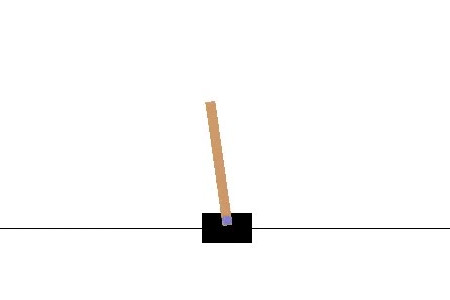
\includegraphics[width=7cm]{cartpole.jpg}
    \caption{The cartpole to balance verticaly. The cartpole can be seen as an inverted pendulum
    sitting on a small moving cart.}
\end{figure}

\begin{enumerate}
    \item Could we tackle this problem without machine learning ? Do you have any idea how ?
    \item Given the state vector of the cart pole, let us keep only 2 features, the angle of the
        pole and the cart velocity. How can you transform those continuous variables to
        categorical ones ? Why do you need to do so ?
    \item What is the reward function of this problem ? What are the possible actions ?
    \item Using Q Learning to solve this problem, what will be the dimensionnality of the Q table.
    \item What is the Bellman equation ? Where is it used in Q learning ?
    \item Using the provided template, implement you solution in python. 

\end{enumerate}

\reponse{
    (a) It could be done using regular control theory (\url{https://en.wikipedia.org/wiki/Inverted_pendulum)}\\

    (b) Create bins of values, since Q learning uses a Qtable we need to be able to categorize so that
    the number of cases in the table in finite. \\

    (c) +1 for each timestep it still balanced \\

    (d) If we keep only 2 features and categorize in 20 bins, and knowing that there are 2 possibles
    actions, the table will be : 20x20x2

    (e) The bellman equation is used to update the Q table at each timestep

    (f) see github for implementation
}

\end{Q}

\noindent
\rule{\textwidth}{0.4pt}
\footnotesize{Found an error? Let us know: \url{https://github.com/iridia-ulb/INFOH410/issues}}

\end{document} 
